\chapter{MQTT Broker redundancy}
\label{intro} 


\abstract{

In the long term, the cities of our world should become smart. One area of ​​smart cities is smart mobility. A lot of data is collected in connected vehicles, which can be relevant in a smart city. In this work an approach is developed with which all data of a vehicle are collected in a local MQTT broker. The collected data is transmitted to an online broker of smart city as required or at regular intervals.
}

\section{Introduction}
\label{sec:1}
A large amount of data comes together in modern cars. Many sensors are distributed throughout the vehicle and record parameters of the environment and of the vehicle itself. Much of this information is only valuable for the assistance systems or vehicle occupants.\\


However, some data can also be of interest for external processing in smart cities. A special application is, for example, sending an emergency call after an accident. The emergency message should then contain all information that could be relevant for the rescue and security measures. Such as: position, number of vehicle occupants, speed before the accident and vehicle condition (fire, oil ...).\\


This work focuses on the data exchange between a vehicle and a smart city server connected via Message Queue Telemtry Transport (MQTT) protocol. A loss of data when the connection is broken is to be excluded.\\


\subsection{MQTT}
Message Queuing Telemetry Transport (MQTT) is an open network protocol for machine-to-machine communication (M2M) that enables the transmission of telemetry data in the form of messages between devices. MQTT is a client-server protocol. Clients connect to the server, also called broker, and can publish messages with a topic. Clients can subscribe to these topics, with the server forwarding the received messages to the corresponding subscribers. Figure \ref{fig:mqtt_overview} shows that clients can be subscribers, publishers, or both.\cite{mqtt_doc}\\

\begin{figure}
\sidecaption
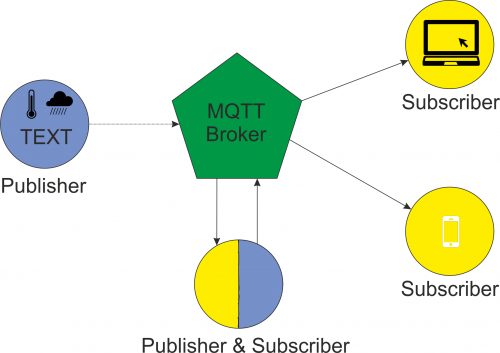
\includegraphics[scale=.5]{images/images_michael/MQTT_Overview-e1520778847225.png}
\caption{MQTT overview\cite{mqtt_overview}}
\label{fig:mqtt_overview}
\end{figure}
\section{Related works}
\label{sec:2}

The research group Schmitt, Carlier and Renault also dealt with redundant brokers. They have developed an approach in which several brokers in a network mirror their data. If a broker crashes in the system, all data is still available and the system is still accessible to the clients.\\

\begin{figure}
\sidecaption
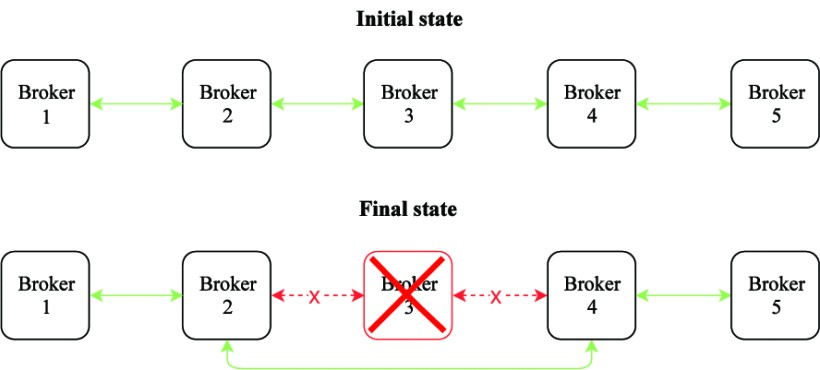
\includegraphics[scale=.5]{images/images_michael/schmi3-p5-schmi-large.jpg}
\caption{Dynamic MQTT Bridge}
\label{fig:bridge}
\end{figure}
Figure \ref{fig:bridge} shows five brokers in a line topology. Each broker mirrors the data of its direct neighbors. For example, once crashes broker three, connect broker two and four and their data mirrored. When broker 3 is online again, it will re-arrange itself and compare its data with the neighboring brokers.\\


\section{Concept}
\label{sec:3}

This project simulates a vehicle that is moving in a smart city. There are some sensors in this vehicle that send the recorded data to a local broker (Figure \ref{fig:req} - Req B in the vehicle. The local broker is also subscriber and publisher to the smart city online broker. The collected data from all sensors should now be forwarded to the online broker at regular intervals. The aim is to guarantee that all data is transmitted reliably and that there is no data loss even if the connection is broken (Figure \ref{fig:req} - Req C).\\


To meet these requirements, all data is collected in a data structure and transferred from the local broker to the online broker when there is an existing connection. To ensure that the data was transmitted correctly, the local broker listens to the data topic and compares the messages. The data structure in the local broker is only reset if the incoming data is identical to the sent data.\\


Since the vehicle is moving, a continuous connection to the online broker cannot be maintained. The system must detect connection drops(Figure \ref{fig:req} - Req A). Until the connection is re-established, all data is collected in the local broker and transmitted when it is reconnected (Figure \ref{fig:req} - Req E).\\

\begin{figure}
\sidecaption
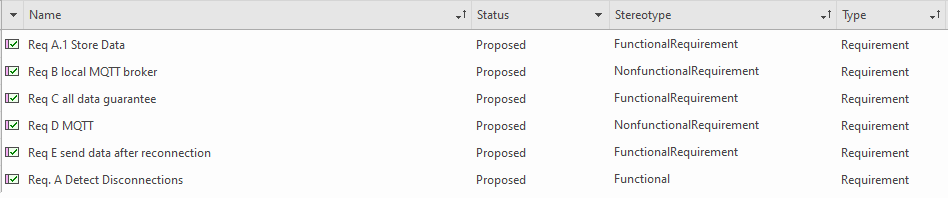
\includegraphics[scale=.5]{images/images_michael/Requirements_list.PNG}
\caption{Requirements table}
\label{fig:req}
\end{figure}

The Sequence Diagram (Figure \ref{fig:sequence}) shows what a message history of the system could look like. The sensor is representative of any number of sensors in the vehicle, which send all their data to the local broker. As long as there is a connection to the online broker, all data will be forwarded by the local broker at regular intervals. After the third transmission, the connection is broken. Only after some time there is again a connection and data transfer is resumed.\\


\begin{figure}
\sidecaption
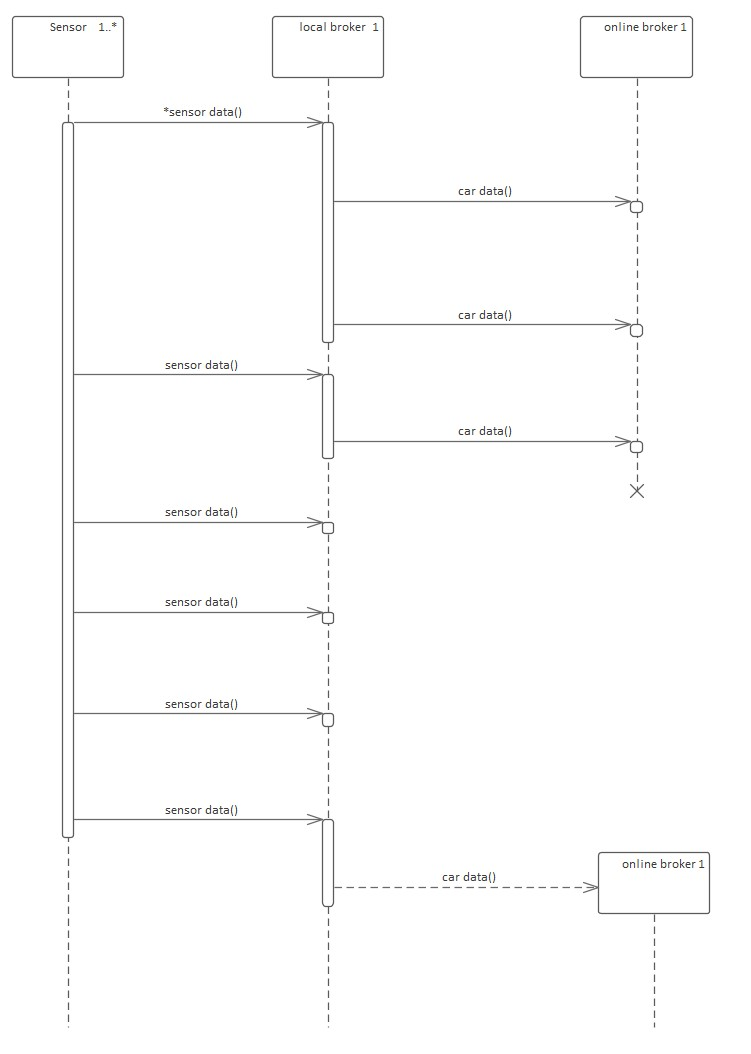
\includegraphics[scale=.5]{images/images_michael/sequence_diagram.jpg}
\caption{sequence diagram}
\label{fig:sequence}
\end{figure}
\begin{figure}
\sidecaption
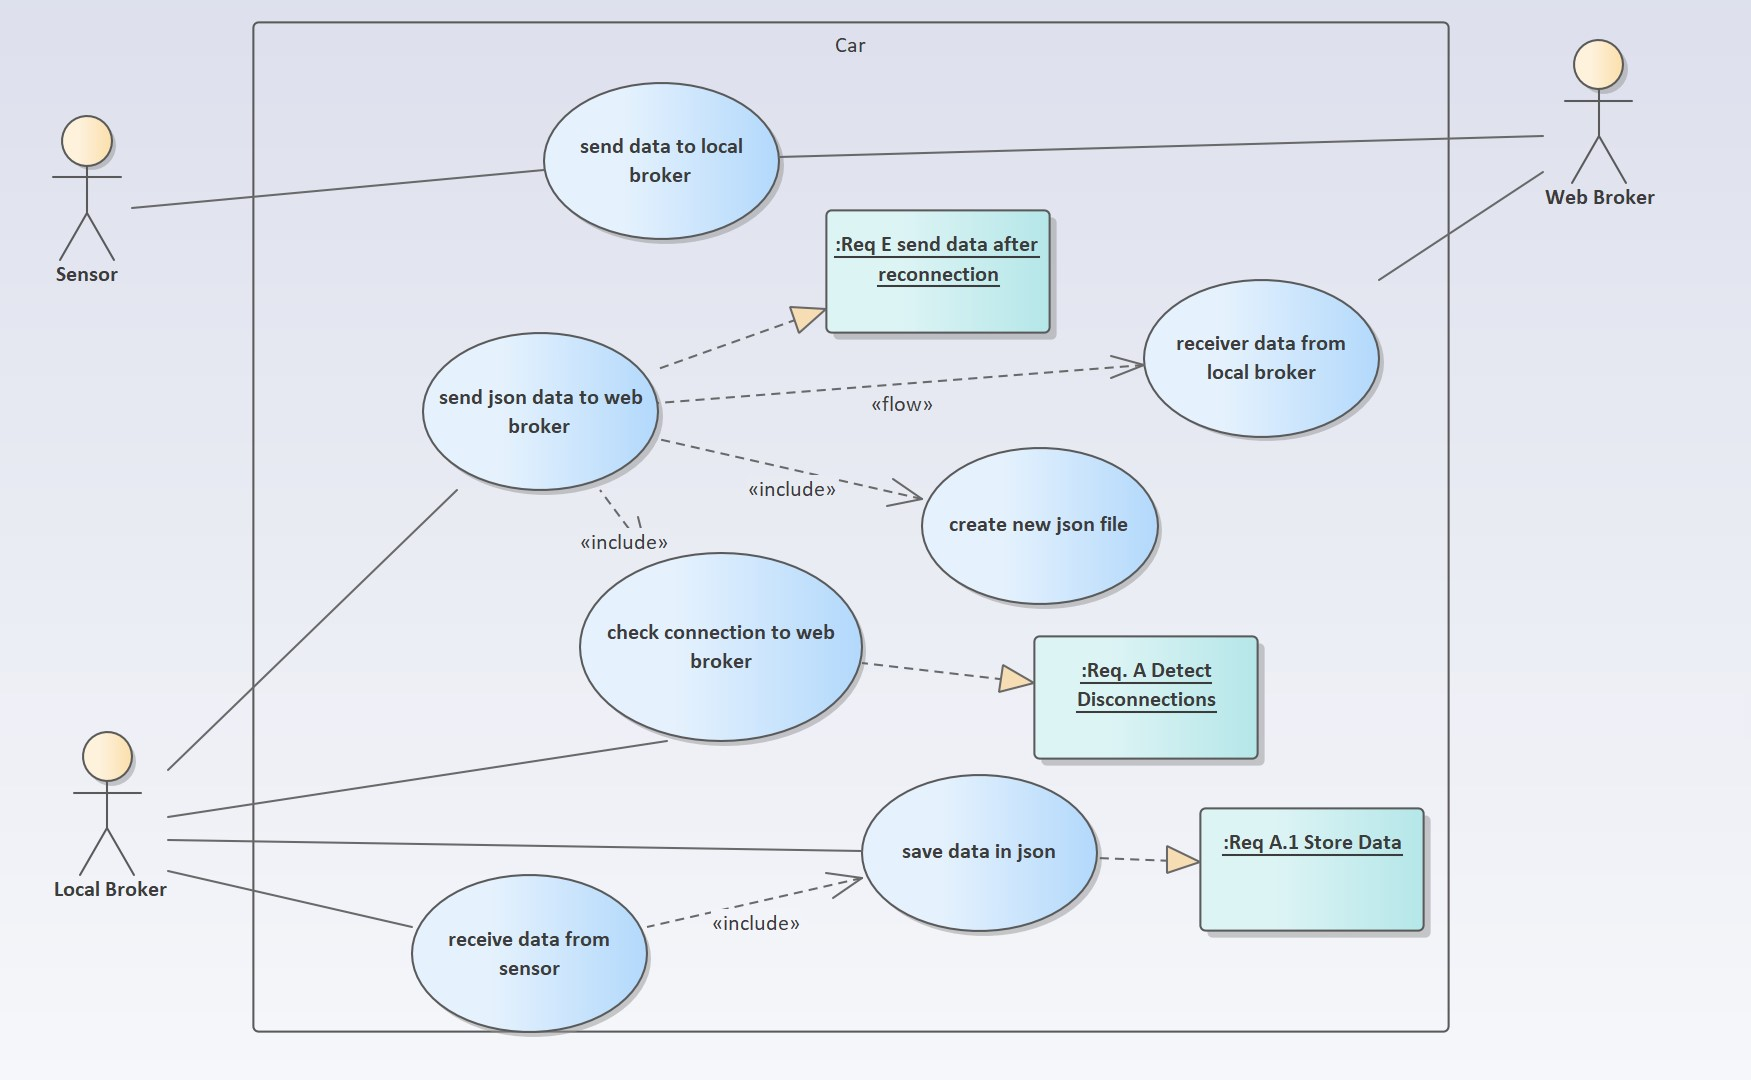
\includegraphics[scale=.25]{images/images_michael/use_case_diagram.jpg}
\caption{use case diagram}
\label{fig:3}
\end{figure}

\section{Implementation}
\label{sec:4}
The system is written in python consists of four sub-programs:

\begin{itemize}
    
    \item GPS
    \item Temperature Sensor
    \item Local broker
    \item Emergency unit
\end{itemize}

The GPS sub-program simulates driving through the city. After starting the program, an array with different coordinates is created. These coordinates represent the route from Figure \ref{fig:route}. The connection to the local broker is then established and the program runs through the coordinate array in a 10-second interval and publishes the current location in the topic $/car/gps$ on the local broker.

\begin{figure}
\sidecaption
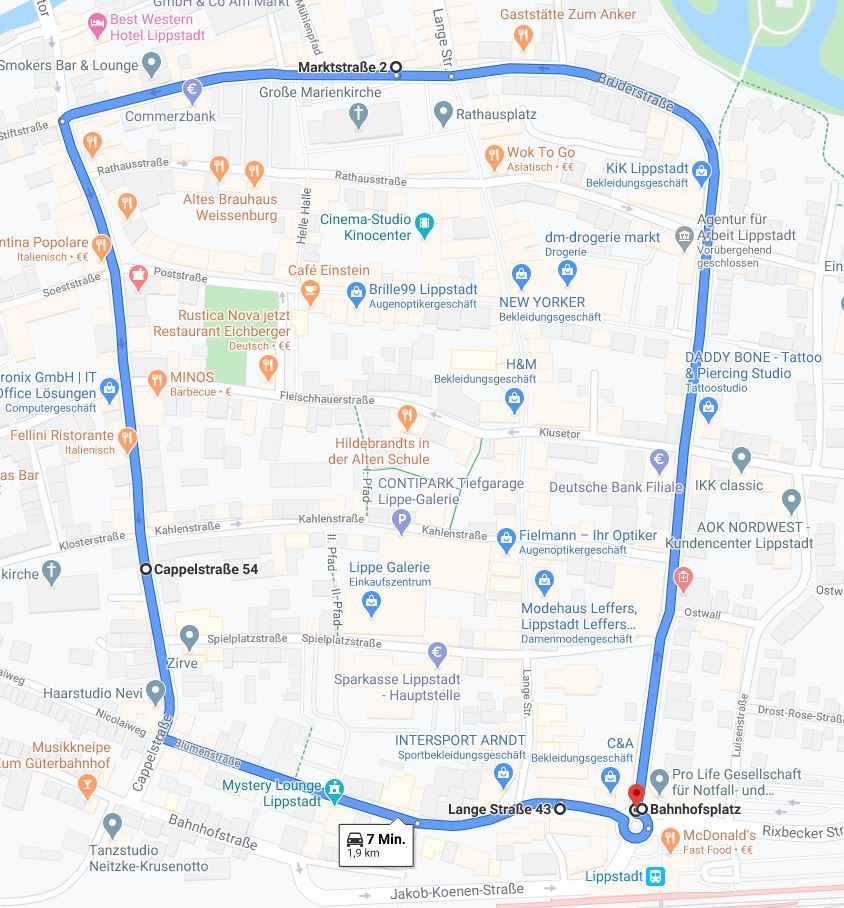
\includegraphics[scale=.4]{images/images_michael/route.JPG}
\caption{circular route through lippstadt.}
\label{fig:route}
\end{figure}

The temperature sensor should be representative of all other sensors installed in a vehicle. After starting the program, he connects to the local broker. Then he publishes every three seconds a random value between 15 and 30 at $/car/temperature$.\\


\begin{figure}
\sidecaption
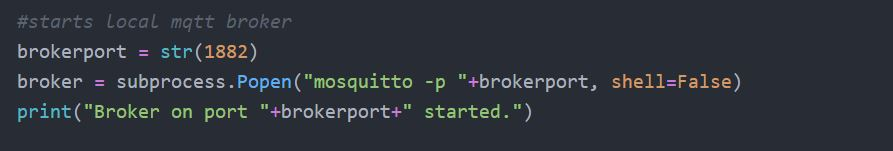
\includegraphics[scale=.5]{images/images_michael/local_broker_start.JPG}
\caption{start local broker}
\label{fig:start_broker}
\end{figure}
 
 The local broker consists of the python program and a mosquitto broker. At the beginning of the program, the mosquitto broker is started (Figure \ref{fig:start_broker}). Then the connection to the online broker and the local mosquitto broker is established. \\
 
 
 In the next step, the vehicle or local broker registers with the server. Figure \ref{fig:register} shows the function created for this. For successful registration, the server must be sent a serialized dictionary with name, position, reasons and id. JSON is used for serialization. The server then creates a personal topic $/hshl/users/id$ on the online broker. From now on, all communication takes place via this topic or its subtopics. The subtopic $/hshl/users/id/data$ is created for the transfer of the sensor data.\\
 
 
\begin{figure}
\sidecaption
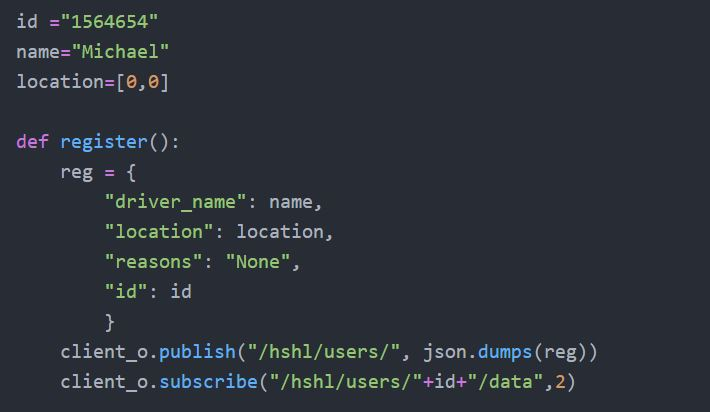
\includegraphics[scale=.5]{images/images_michael/register_function.JPG}
\caption{register function}
\label{fig:register}
\end{figure}

After registration there are two main functions. On the one hand, there is an endless loop in which the collected sensor data is sent to the online broker every 8 seconds (Figure \ref{fig:6}). Figure \ref{fig:7} shows the function $on\_message\_online$. This function is called as soon as a message arrives from the online broker. If the message was published on the data topic, it is checked whether it is identical to the collected sensor data. This makes it possible to determine whether all data has been transferred correctly. In the positive case, the data structure is emptied in order not to send the same data records multiple times.\\


\begin{figure}
\sidecaption
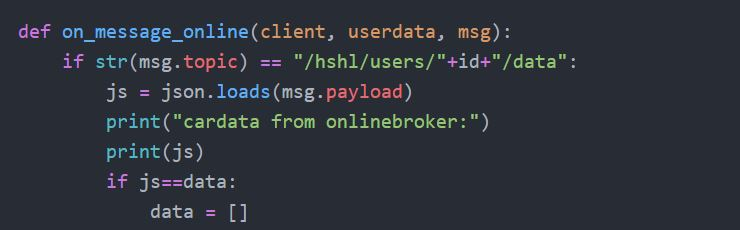
\includegraphics[scale=.5]{images/images_michael/data_message.JPG}
\caption{data message}
\label{fig:7}
\end{figure}

On the other hand there is the request function (Figure \ref{fig:5}). This is called up as soon as a message in the topic reason arrives at the local broker. The emergency unit is used for this function. The emergency unit can send various reasons to the local broker (Figuire \ref{fig:6}). The reasons can be selected by the user. These are forwarded to the server by the request function. The server evaluates the reasons and notifies the relevant institutions (see Chapter 2).\\


\begin{figure}
\sidecaption
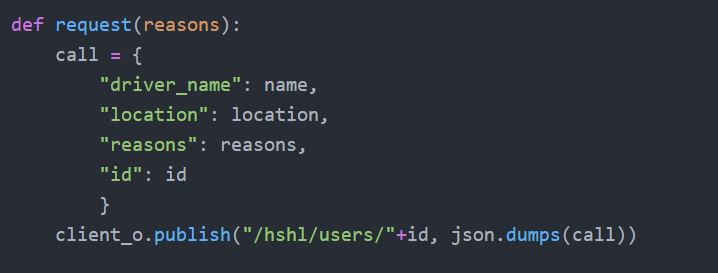
\includegraphics[scale=.5]{images/images_michael/request_function.JPG}
\caption{request function}
\label{fig:5}
\end{figure}

\begin{figure}
\sidecaption
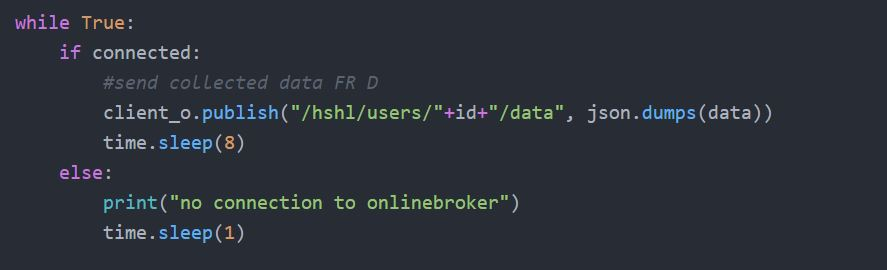
\includegraphics[scale=.5]{images/images_michael/main_loop.JPG}
\caption{main loop}
\label{fig:6}
\end{figure}



\begin{figure}
\sidecaption
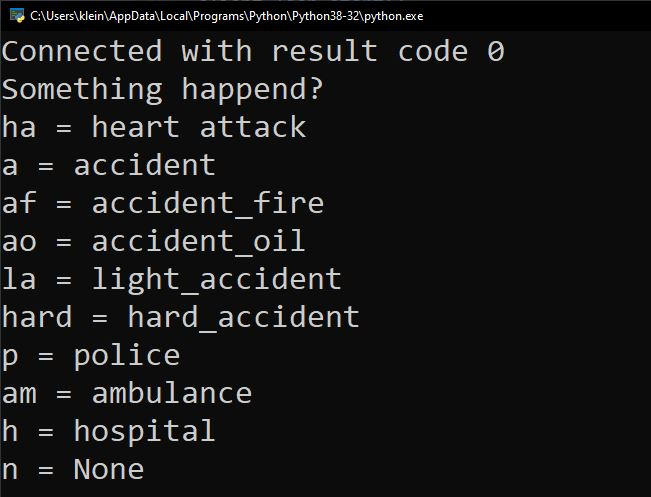
\includegraphics[scale=.5]{images/images_michael/reasons.JPG}
\caption{reasons}
\label{fig:8}
\end{figure}
   

\section{Results}
\label{sec:5}
In this project, an approach to data transfer between vehicles and smart cities was developed. All the requirements set out in the figure could be implemented. Handling of emergency calls could be improved in the future. For example, it would be good if these were also saved until they were guaranteed to be transmitted to the server. Furthermore, emergency calls should be discarded after a certain time without transmission, as they will probably no longer be relevant at some point.



\newpage
\bibliographystyle{IEEEtran}
\bibliography{./chapter.bib}